\tikzstyle{highlightGreen}=[line width=1.5pt,draw=green]
\begin{frame}[fragile]
\begin{overlayarea}{\textwidth}{15cm} 
\begin{tikzpicture}[remember picture,line width=1.5pt,]
\tikzset{
mybox/.style = {draw=red, fill=yellow!50, very thick,
    rectangle, rounded corners, inner sep=2pt, inner ysep=4pt}
}
\node[draw=black,temporal=<2>{fvisible}{highlightGreen}{semivisible},text width=0.45\textwidth,inner sep=0pt](a)
{%
\begin{minipage}[t]{\textwidth}%
\noindent
\begin{lstlisting}[language=C,escapechar=~]
#include<assert.h>
void main()
{
  int i_s,x_s,y_s,n,out_s;
  int i_t,x_t,y_t,out_t;
  __CPROVER_assume(n>=0);
  assert(!(n>=0));
\end{lstlisting}
\end{minipage}};
\node[draw=black,temporal=<3>{fvisible}{highlightGreen}{semivisible},onslide=<2>{semivisible},below=of a,text width=0.45\textwidth,inner sep=0pt,yshift=0.8cm] (b){%
\begin{minipage}{\textwidth}%
\noindent
\begin{lstlisting} [language=C,escapechar=~,firstnumber=8]
// cTrace for M0
  if(n>=0)
  {
    i_s=0;x_s=0;y_s=0;
    __CPROVER_assume(i_s<=n);
    assert(!(i_s<=n));
    while(i_s<=n)
    {
      x_s=5;
      y_s=y_s+5;
      i_s=i_s+1;
    }
    out_s=x_s+y_s;
  }
\end{lstlisting}
\end{minipage}};
\node[draw=black,temporal=<4>{fvisible}{highlightGreen}{semivisible},onslide=<2-3>{semivisible},right=of b,text width=0.47\textwidth,inner sep=1pt,yshift=3cm] (c){%
\begin{minipage}{\textwidth}%
\noindent
\begin{lstlisting} [language=C,escapechar=~,firstnumber=22]
//cTrace for M1
  if(n>=0)
  {
    i_t=0;x_t=0;y_t=0;
    __CPROVER_assume(i_t<=n);
    assert(!(i_t<=n));
    while(i_t<=n)
    {
      y_t=y_t+5;
      i_t=i_t+1;
    }
    x_t=5;
    out_t=x_t+y_t+1;
  }
\end{lstlisting}
\end{minipage}};
\node[draw=black,temporal=<5>{fvisible}{highlightGreen}{semivisible},onslide=<2-4>{semivisible},below=of c,text width=0.47\textwidth,yshift=0.8cm,inner sep=1pt] (d) 
{%
\begin{minipage}{\textwidth}%
\noindent
\begin{lstlisting}[language=C,escapechar=~,firstnumber=36]
//Live variables
  assert(x_s = x_t);
  assert(y_s = y_t);
//Output variable
 assert(out_s = out_t);
}
\end{lstlisting}
\end{minipage}};

\node[temporal=<2>{invisible}{fvisible}{invisible},mybox,below=of c,xshift=-3cm,yshift=3cm,text width=10cm]
{\begin{minipage}{\textwidth}
\begin{itemize}
\item \_s -- Variables appearing in the cTrace of $M_0$.
\item \_t -- Variables appearing in the cTrace of $M_1$.
\item n -- common Variable.
\item $\mathtt{\_\_CPROVER\_assume}$ -- allow only those computations that satisfy a given condition.
\end{itemize}\end{minipage}};

\node[temporal=<3>{invisible}{fvisible}{invisible},mybox,inner sep=0pt,right=of b,yshift=2cm,xshift=-0.45cm]
{\begin{minipage}[t]{0.5\textwidth}
\linespread{1.5}
\begin{tikzpicture}[line width=1.5pt,place/.style={circle,draw}]
        %%%%%%%%%%%%%%%%%%%%%%%%%%%M0%%%%%%%%%%%%%%%%%%%%%%
          \node[fill=gray!20] (1) at (0,1)   [place] {$q_{00}$};
          \node[fill=gray!20] (2) at (0,-2)   [place] {$q_{01}$};
          \node (3) at (-1.5,-5)   [place] {$q_{02}$};
          \node (5) at (1.5,-5)   [place] {$q_{03}$};
          
          \draw [>=latex,->,draw=green](1) to [align=center] node[pos=0.5,left] 
          {\footnotesize $n\geq 0/$\\[-0.3cm] \footnotesize $i\Leftarrow 
          0,$\\[-0.3cm]\footnotesize $x\Leftarrow 0,$\\[-0.3cm]\footnotesize 
          $y\Leftarrow 0$} 
          node[pos=0.4,right]{$p_{01}$} (2);
          
          \draw [>=latex,->,draw=yellow](2)  [align=center] to  
          node[pos=0.6,right] {\footnotesize$i\leq n/$\\[-0.2cm]\footnotesize 
          $\boxed{\mathbf{x\Leftarrow 5}},$\\[-0.3cm]\footnotesize $y\Leftarrow 
          y+5$}(3);
          
          \draw [>=latex,->, draw=yellow](3) [align=center] .. controls (-3,-2) 
          and (-0.8,-2) ..  node[pos=0.3,left] 
          {\rotatebox[origin=c]{90}{\footnotesize -/\footnotesize$i\Leftarrow 
          i+1$}}  node[pos=0.3,right,xshift=0.3cm]{$p_{02}$}(2);
          
          \draw [>=latex,->,draw=red](2)  [align=center] 
          --node[pos=0.5,right]{\footnotesize$\neg i\leq 
          n/$\\[-0.2cm]\footnotesize{\boxed{\mathbf{out\Leftarrow x+y}}}}
          node[pos=0.8,right]{$p_{03}$}(5);       
        \end{tikzpicture}
\end{minipage}};

\node[temporal=<4>{invisible}{fvisible}{invisible},mybox,inner sep=0pt,left=of d,yshift=3cm,xshift=0.7cm]
{\begin{minipage}[t]{0.5\textwidth}
\linespread{1.5}
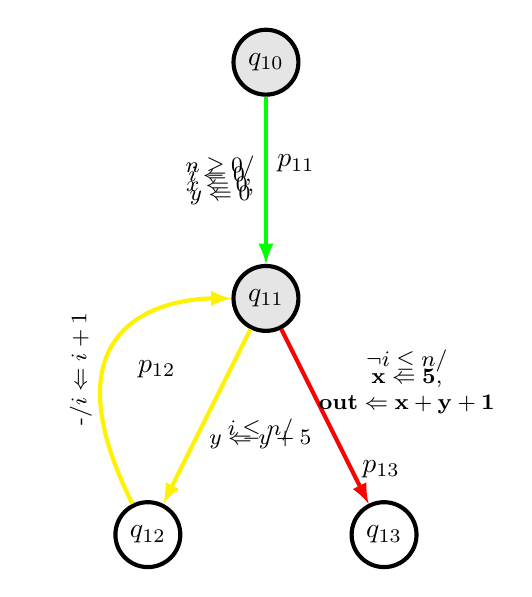
\begin{tikzpicture}[line width=1.5pt,place/.style={circle,draw}]
        %%%%%%%%%%%%%%%%%%%%%%%%%%%M0%%%%%%%%%%%%%%%%%%%%%%
          \node[fill=gray!20] (1) at (0,1)   [place] {$q_{10}$};
          \node[fill=gray!20] (2) at (0,-2)   [place] {$q_{11}$};
          \node (3) at (-1.5,-5)   [place] {$q_{12}$};
          \node (5) at (1.5,-5)   [place] {$q_{13}$};
          
          \draw [>=latex,->,draw=green](1) to [align=center] node[pos=0.5,left] 
          {\footnotesize $n\geq 0/$\\[-0.3cm] \footnotesize $i\Leftarrow 
          0,$\\[-0.3cm]\footnotesize $x\Leftarrow 0,$\\[-0.3cm]\footnotesize 
          $y\Leftarrow 0$}
          node[pos=0.4,right]{$p_{11}$}
          (2);
          
          \draw[>=latex,->,draw=yellow](2)  [align=center] to  
          node[pos=0.6,right] {\footnotesize$i\leq n/$\\[-0.3cm]\footnotesize 
          $y\Leftarrow y+5$}(3);
          
          \draw [>=latex,->,draw=yellow](3) [align=center] .. controls (-3,-2) 
          and (-0.8,-2) ..  
          node[pos=0.3,left] {\rotatebox[origin=c]{90}{\footnotesize 
          -/\footnotesize$i\Leftarrow i+1$}}
          node[pos=0.3,right,xshift=0.3cm]{$p_{12}$}(2);
          
          \draw [>=latex,->,draw=red](2)  [align=center] 
          --node[pos=0.3,right,]{\footnotesize$\neg i\leq 
          n/$\\[-0.2cm]\footnotesize $\boxed{\mathbf{x\Leftarrow 
          5}},$\\[-0.1cm]\footnotesize
          ${\boxed{\mathbf{out\Leftarrow x+y+1}}}$}
          node[pos=0.8,right]{$p_{13}$}
          (5);
        \end{tikzpicture}
\end{minipage}};
\node[temporal=<5>{invisible}{fvisible}{invisible},mybox,above=of d,xshift=-3cm,yshift=1cm,text width=10cm]
{\begin{minipage}{\textwidth}
\begin{itemize}
\item CBMC verifies the specified assertions. 
\item If any violation of an assertion is detected, a counter-example is
generated.
\item $n = 0$ the values of the variable `out' differs.
\end{itemize}\end{minipage}};

\end{tikzpicture}
\end{overlayarea}
\end{frame}
